\section{Final new-source mechanism confirmation}
An earlier three-source parameter-matched confirmation produced an activation-by-correctness interaction of 14.71 pp [9.51,20.05]. Posthoc predicted-null swaps and adequately fitted affine diagnostics on those same sources motivated the present hypotheses; a fresh-input check on reused sources is not new-source confirmation. We do not pool these exploratory and prior-confirmation outcomes with the final experiment.

We fixed this as the last experimental round before observing its new outcomes. Five previously unused source seeds (17291, 18401, 19507, 20611, 21713) were trained from scratch for 500 ordinary epochs and 900 correct single-generator preparation epochs. No old source checkpoint was reused. The five encoders, original maps and readouts were then frozen. Each source has its own 1024-anchor first-operator support, while the new source corpus and test are shared. Supports may overlap; source/validation/support/test complete group orbits are separated within the study. The new test excludes all 2688 previously examined matrix test orbits and contains 256 IID examples and 128 collision pairs. Historical inputs can recur in the new training partitions under new initialized models.

\paragraph{Matched activation and correspondence.}
Two-layer Identity and GELU first-operator residuals have identical width 256 and 65,920 trainable parameters, fixed original affine skip connections, matching initialization and zero final layers. Correct teacher logits, start states, schedules and 2000 AdamW updates are shared. Wrong geometry uses a complete derangement preserving all three visible gold answers. All four first-operator arms use zero weight decay, declared before fitting, to match the unregularized data objective of the convergence diagnostic. This harmonization differs from the earlier 0.0001-decay confirmation; the earlier results remain unchanged. The scalar encoder and source-preparation protocol are unchanged.

\paragraph{Predicted null-component transfer.}
For two predicted first states $\hat h_L,\hat h_G$ in the same source coordinates, with $P$ the row projector of the frozen full linear readout, we construct
\[
\hat h_{L\leftarrow G}=\hat h_L P+\hat h_G(I-P).
\]
The intervention uses no true intermediate state. It preserves every first-step logit, not only the winning class. Correct and matched-wrong GELU donors and reverse transfer are reported. Correct-null transfer yields +8.75 pp [+5.31,+12.42] improvement on collision AB; the correct-minus-wrong donor contrast is +8.44 pp [+4.92,+11.95]. Across interventions the maximum logit change is $2.23\times10^{-13}$. This tests a functional pathway in the specified frozen composition; hybrid states need not lie on the encoder manifold and the intervention does not remove all answer information.

\paragraph{Same-family, same-loss affine convergence.}
The two-layer Identity residual can express an unrestricted affine map. We solve exactly its shared empirical loss,
\[
 L(R)=\mathrm{KD}_{T=2}(R(h_0)W^\top+b_W,z_A)+0.25\,\frac{\|R(h_0)-h_A^{\mathrm{paired}}\|_F^2}{Nds^2},
\]
with $s^2$ fixed from correct training targets and the identical stored teacher logits $z_A$ used in all arms. There are no compound targets, ridge terms or validation-selected geometry weights. Float64 SVD whitening conditions the affine training design; readout-null coefficients have the exact least-squares solution, and readout-row coefficients are optimized by L-BFGS. Both OLS and original budget-linear row initializations are fixed in advance. The strongly convex quadratic term permits a gradient-based upper bound on remaining training-objective error. Independent analytic full gradients verify every solution. Both initializations, coefficient norms, condition numbers and float32-versus-float64 inference are retained. Changed parameterization, precision and additional budget are optimization diagnostics, not another equal-budget intervention.

\begin{table}[ht]\centering\small
\begin{tabular}{lrrr}\toprule First operator & Collision AB (\%) & Both correct (\%) & First-state NMSE\\\midrule
linear correct & 8.44 & 0.47 & 0.04647 \\
linear wrong & 9.45 & 0.31 & 0.06859 \\
nonlinear correct & 20.31 & 5.00 & 0.01973 \\
nonlinear wrong & 8.44 & 1.09 & 0.06874 \\
converged correct & 19.92 & 3.75 & 0.02963 \\
converged wrong & 8.36 & 0.31 & 0.08200 \\
\bottomrule\end{tabular}
\caption{Final five-source confirmation, with original budget-controlled arms and separately budgeted converged affine diagnostics. All predictions begin from the input representation and use the frozen second operator.}\end{table}

\paragraph{Predeclared contrasts.}
The same-budget activation-by-correctness interaction is +12.89 pp [+8.67,+17.03]. After affine convergence, the remaining GELU-versus-affine relation-advantage interaction is +0.31 pp [-5.86,+6.33]. Intervals resample five independent source clusters and the 128 common collision pairs; individual-source effects are provided in the experiment artifacts. These are descriptive intervals for separately stated hypotheses, not familywise-adjusted significance tests. Crossing zero cannot establish equivalence. All source gates and convergence checks are retained, without replacement of unfavorable sources.

\paragraph{Convergence and numerical qualification.}
The largest independently recomputed training-objective gap bound is $3.87\times10^{-12}$. Both fixed initializations yield identical compound classes, with a maximum predicted first-state difference of $6.55\times10^{-5}$. However, the affine design is ill-conditioned: condition numbers range from $8.65\times10^{7}$ to $1.29\times10^{8}$, and coefficient Frobenius norms range from $8.01\times10^{5}$ to $1.69\times10^{6}$. Replaying the complete affine--second-operator--readout pipeline in float32 changes 12/1280 correct-pairing and 43/1280 wrong-pairing collision predictions relative to float64. Aggregate correct/wrong accuracies are 19.92/8.36\% in float64 and 19.92/8.44\% in float32. Thus the main aggregate correctness advantage remains under this precision check, while individual predictions and high-norm coefficients are numerically sensitive. The convergence certificate concerns the finite empirical objective; it does not guarantee perturbation robustness or generalization to arbitrary inputs.

\begin{figure}[ht]\centering
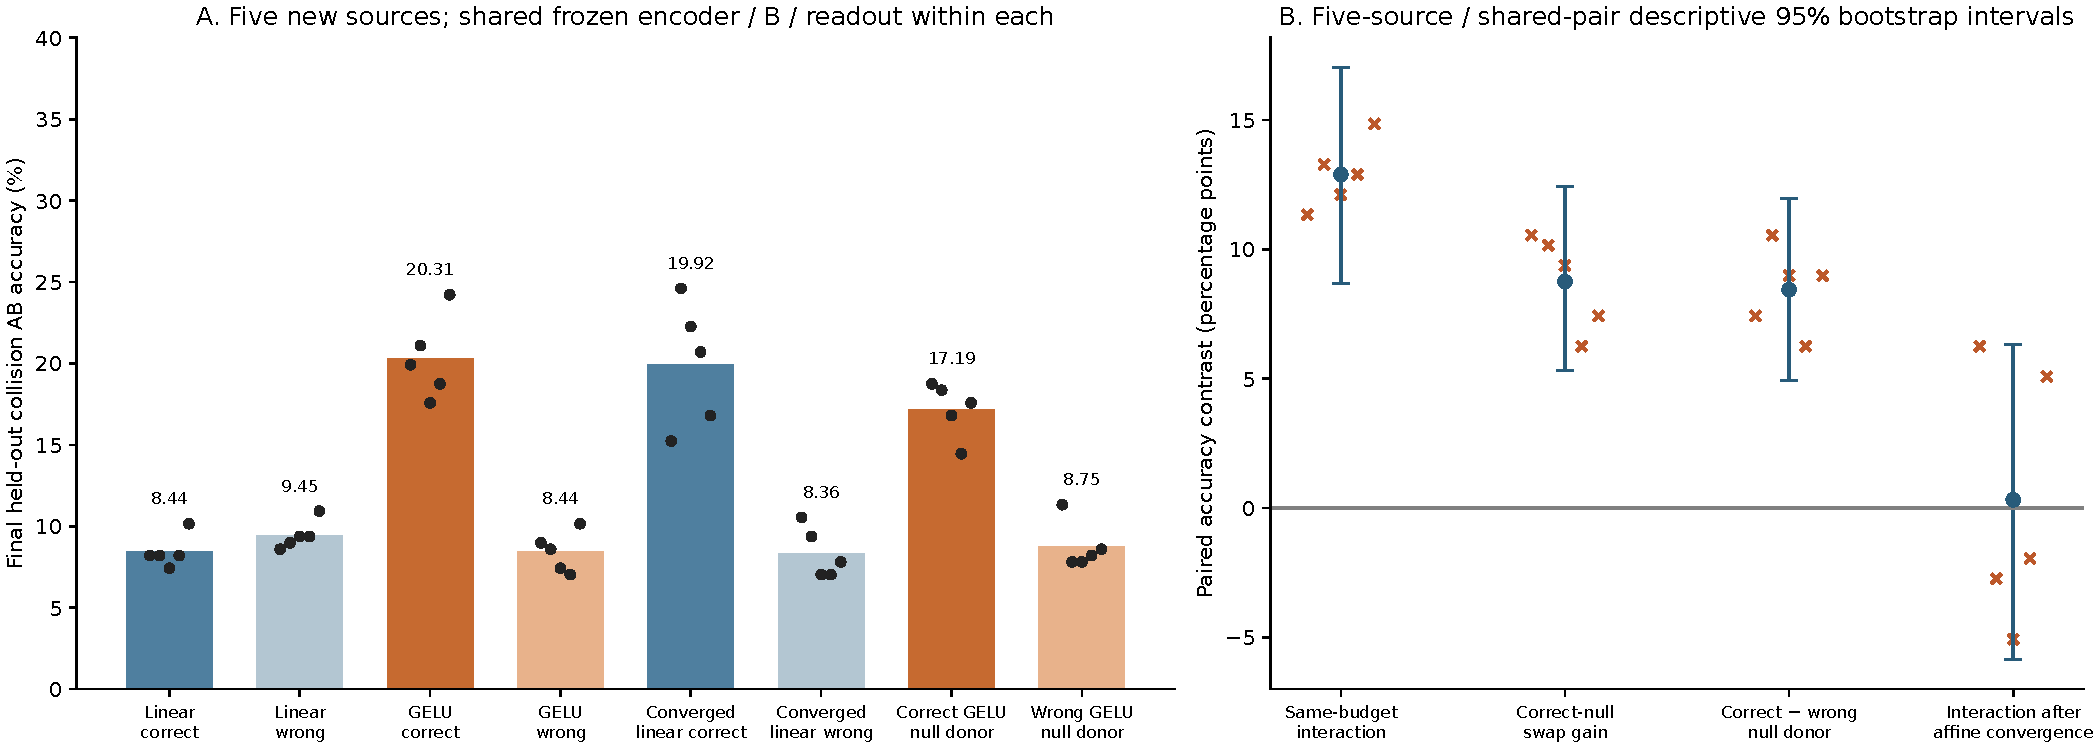
\includegraphics[width=\linewidth]{../results/final_mechanism_confirmation/final_confirmation.pdf}
\caption{Final confirmation with five new source initializations, predicted-component transfer, and the predeclared same-loss convergence diagnostic. Points show all five sources.}\end{figure}

\paragraph{Closing interpretation.}
We did not confirm an additional expressivity advantage in functional relation-specific composition after adequate affine fitting. State-fitting differences and unresolved numerical and optimization explanations are retained as limitations. We do not assign exact percentage contributions to optimization, numerical conditioning and expressivity. No additional domains, source seeds, losses or mechanistic training schemes are added after this fixed confirmation. The remaining work is manuscript refinement and submission preparation.
